\chapter{結論}
\label{conclusion}

本章では,本研究の総括と今後の課題を示す.

\section{本研究のまとめ}
% 本研究では,IPv6シングルスタックネットワークにおけるIPv4サービス提供手法として,"SIIT-DC"と呼ばれるネットワークデザインに着目した.SIIT-DCでは,BRと呼ばれるプロトコル変換機構を有したルータが,アドレス変換テーブル(EAMT)を参照してIPv4/IPv6トランスレーションを行い,IPv6サーバでIPv4サービスの提供を可能にする.
% SIIT-DCのアーキテクチャにおいて,複数のBRを運用する環境でのEAMTの一貫性の確保が難しい点や,IPv4でサービス提供を行うサーバの構成変更が行われた際に個別の運用が必要になる点を課題として示した.また,SIIT-DCのこれらの問題を解決するためには,BRが保有するEAMTを動的に制御する”ダイナミックEAMT機構”が必要となることを指摘した.

% ダイナミックEAMT機構を実現する手法に関して,中央管理型アプローチと分散管理型アプローチを比較し,それらのメリットを兼ね揃えた手法動的経路制御プロトコルであるBGPを利用した手法を考案した.BGPではノード間で一定の経路情報の一貫性を保証するほか,BGPピアの状態の変化にダイナミックに対応した制御を行う事ができる.本提案手法では,IBGPをEAMT管理機構に適応するための機能拡張を行うと共に,ルートリフレクタを利用したスケーラブルなダイナミックEAMT管理・制御機構を実現した.


% 本手法を評価するために,OSS及び自作のEAMT制御機構を利用した概念検証実装を作成し2つのシナリオからなる評価実験を行った.本評価実験の結果,本手法が30台のBR,2台のルートリフレクタ,最大600台のサーバからなる評価用ネットワークにおいて,ダイナミックEAMTを実現するために十分なフィジビリティを有することが明らかになった.

% \section{よりスケーラブルなBGPコネクショントポロジについての検討}
% \label{conclusion:tree}
% 本評価実験を通して,ルートリフレクタが保有するべきBGPコネクションの数が大きくなることが,IPv4サービス提供サーバの収容可能台数と変更追従性に影響を及ぼすことがわかっている.

% BGPコネクショントポロジを多層のルートリフレクタ構成を用いることによりスケーラブルに本提案手法を運用することが可能である.
% 本節では2層のツリー型トポロジで接続されたルートリフレクタ群のスケーラビリティを定式化し,本提案手法の潜在的なスケーラビリティを明らかにする.

% \subsection{2層のツリー型コネクショントポロジ}
% \label{conclusion:tree:2layer}
% 本項では,ツリー型トポロジによるルートリフレクタの多層化により,ネットワーク全体で収容可能なサーバ台数を拡大するBGPコネクション設計を提案する.

% 本提案において,ルートリフレクタの多層化とは,ルートリフレクタ間でツリートポロジ型のコネクションを確立させるようにルートリフレクタを配置する手法と定義する.

% 2層のツリー型トポロジで接続されたSIIT-DCの各ノードの関係図\ref{fig:2layer_bgp_topology}に示す.BRとコネクションを接続するルートリフレクタを第一層,サーバとコネクションを接続するルートリフレクタを第二層とする.

% このツリー型トポロジではIPv4サービス提供サーバ・ルートリフレクタ・BR間の冗長コネクション数を2として設計している.本トポロジにおいて,IPv4サービス提供サーバ及び各BRが確立するBGPコネクションは2となる.

% \begin{figure}[h]
%     \begin{center}
%     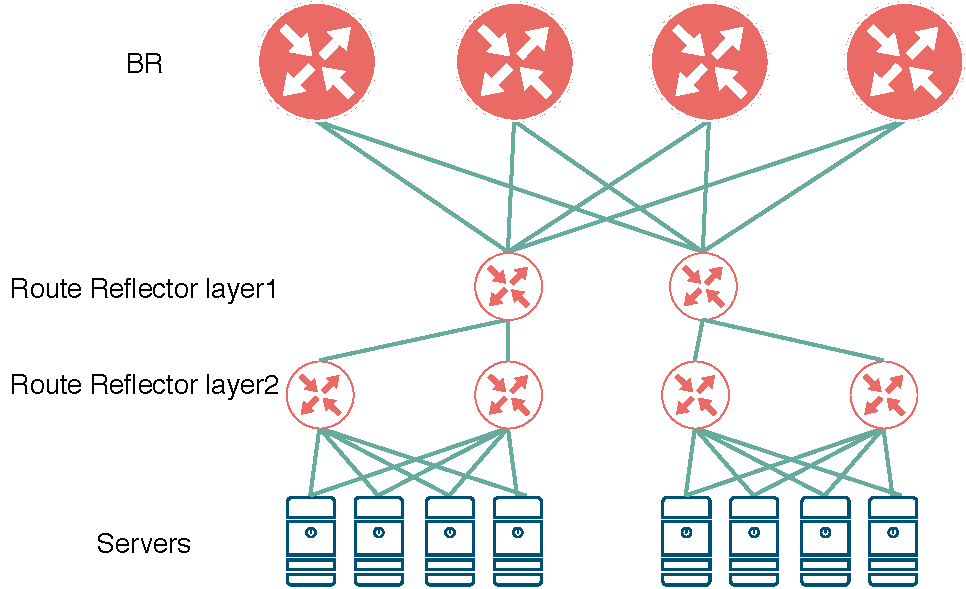
\includegraphics[width=12cm,pagebox=cropbox,clip]{img/2layer_bgp_topology_more_scale.pdf}
%     \end{center}
%     \caption{2層のBGPコネクショントポロジ}
%     \label{fig:2layer_bgp_topology}
% \end{figure}


% また,本トポロジを採用したIDCネットワークにおける収容可能なサーバ数$S$は式\ref{eq:2layer_max_connection}のように示すことが出来る.この時,第一層のルートリフレクタの台数を2,BRのホスト数を$N$,第二層のルートリフレクタの台数を$L$,1台のルートリフレクタが収容可能なBGPピアの最大の数を$C_r$とする.


% \begin{equation}
%     S = \frac{L(C_r - N)}{2} \quad (L \leq C_r - N)
%     \label{eq:2layer_max_connection}
% \end{equation}


% 本研究において行った評価実験環境と同様に,1台のルートリフレクタが収容可能なBGPピア数$C_r$が630,BRの台数$N$が30である場合,本トポロジの最大収容可能サーバ数$S$は180000となる.

% このようにBGPコネクショントポロジを多層化することで,BR及びIPv4サービス提供サーバが確立すべきコネクション数を増やすことなく,本提案手法のスケーラビリティをより高める事が可能になることがわかる.
% 同時に,本提案手法は数万台規模のサーバを抱える実際の商用ネットワークにおいても,本提案手法は高いスケーラビリティを有するモデルであると評価することが出来る.



% \subsection{EAMの集約}
% 本提案手法では,IPv4サービス提供サーバ自身がIPv4サービスアドレスを広告することを前提とした設計を行った.
% IPv4サービスアドレスを有するサーバ以外がEAMを複数集約して代理に広告するというユースケースを想定すると,BGPが利用するアドレスファミリの拡張仕様の設計が必要になると言える.


%%% Local Variables:
%%% mode: japanese-latex
%%% TeX-master: "../thesis"
%%% End:
